% Options for packages loaded elsewhere
\PassOptionsToPackage{unicode}{hyperref}
\PassOptionsToPackage{hyphens}{url}
%
\documentclass[
  man,floatsintext]{apa7}
\usepackage{amsmath,amssymb}
\usepackage{iftex}
\ifPDFTeX
  \usepackage[T1]{fontenc}
  \usepackage[utf8]{inputenc}
  \usepackage{textcomp} % provide euro and other symbols
\else % if luatex or xetex
  \usepackage{unicode-math} % this also loads fontspec
  \defaultfontfeatures{Scale=MatchLowercase}
  \defaultfontfeatures[\rmfamily]{Ligatures=TeX,Scale=1}
\fi
\usepackage{lmodern}
\ifPDFTeX\else
  % xetex/luatex font selection
\fi
% Use upquote if available, for straight quotes in verbatim environments
\IfFileExists{upquote.sty}{\usepackage{upquote}}{}
\IfFileExists{microtype.sty}{% use microtype if available
  \usepackage[]{microtype}
  \UseMicrotypeSet[protrusion]{basicmath} % disable protrusion for tt fonts
}{}
\makeatletter
\@ifundefined{KOMAClassName}{% if non-KOMA class
  \IfFileExists{parskip.sty}{%
    \usepackage{parskip}
  }{% else
    \setlength{\parindent}{0pt}
    \setlength{\parskip}{6pt plus 2pt minus 1pt}}
}{% if KOMA class
  \KOMAoptions{parskip=half}}
\makeatother
\usepackage{xcolor}
\usepackage{graphicx}
\makeatletter
\def\maxwidth{\ifdim\Gin@nat@width>\linewidth\linewidth\else\Gin@nat@width\fi}
\def\maxheight{\ifdim\Gin@nat@height>\textheight\textheight\else\Gin@nat@height\fi}
\makeatother
% Scale images if necessary, so that they will not overflow the page
% margins by default, and it is still possible to overwrite the defaults
% using explicit options in \includegraphics[width, height, ...]{}
\setkeys{Gin}{width=\maxwidth,height=\maxheight,keepaspectratio}
% Set default figure placement to htbp
\makeatletter
\def\fps@figure{htbp}
\makeatother
\setlength{\emergencystretch}{3em} % prevent overfull lines
\providecommand{\tightlist}{%
  \setlength{\itemsep}{0pt}\setlength{\parskip}{0pt}}
\setcounter{secnumdepth}{-\maxdimen} % remove section numbering
% Make \paragraph and \subparagraph free-standing
\makeatletter
\ifx\paragraph\undefined\else
  \let\oldparagraph\paragraph
  \renewcommand{\paragraph}{
    \@ifstar
      \xxxParagraphStar
      \xxxParagraphNoStar
  }
  \newcommand{\xxxParagraphStar}[1]{\oldparagraph*{#1}\mbox{}}
  \newcommand{\xxxParagraphNoStar}[1]{\oldparagraph{#1}\mbox{}}
\fi
\ifx\subparagraph\undefined\else
  \let\oldsubparagraph\subparagraph
  \renewcommand{\subparagraph}{
    \@ifstar
      \xxxSubParagraphStar
      \xxxSubParagraphNoStar
  }
  \newcommand{\xxxSubParagraphStar}[1]{\oldsubparagraph*{#1}\mbox{}}
  \newcommand{\xxxSubParagraphNoStar}[1]{\oldsubparagraph{#1}\mbox{}}
\fi
\makeatother
% definitions for citeproc citations
\NewDocumentCommand\citeproctext{}{}
\NewDocumentCommand\citeproc{mm}{%
  \begingroup\def\citeproctext{#2}\cite{#1}\endgroup}
\makeatletter
 % allow citations to break across lines
 \let\@cite@ofmt\@firstofone
 % avoid brackets around text for \cite:
 \def\@biblabel#1{}
 \def\@cite#1#2{{#1\if@tempswa , #2\fi}}
\makeatother
\newlength{\cslhangindent}
\setlength{\cslhangindent}{1.5em}
\newlength{\csllabelwidth}
\setlength{\csllabelwidth}{3em}
\newenvironment{CSLReferences}[2] % #1 hanging-indent, #2 entry-spacing
 {\begin{list}{}{%
  \setlength{\itemindent}{0pt}
  \setlength{\leftmargin}{0pt}
  \setlength{\parsep}{0pt}
  % turn on hanging indent if param 1 is 1
  \ifodd #1
   \setlength{\leftmargin}{\cslhangindent}
   \setlength{\itemindent}{-1\cslhangindent}
  \fi
  % set entry spacing
  \setlength{\itemsep}{#2\baselineskip}}}
 {\end{list}}
\usepackage{calc}
\newcommand{\CSLBlock}[1]{\hfill\break\parbox[t]{\linewidth}{\strut\ignorespaces#1\strut}}
\newcommand{\CSLLeftMargin}[1]{\parbox[t]{\csllabelwidth}{\strut#1\strut}}
\newcommand{\CSLRightInline}[1]{\parbox[t]{\linewidth - \csllabelwidth}{\strut#1\strut}}
\newcommand{\CSLIndent}[1]{\hspace{\cslhangindent}#1}
\ifLuaTeX
\usepackage[bidi=basic]{babel}
\else
\usepackage[bidi=default]{babel}
\fi
\babelprovide[main,import]{english}
% get rid of language-specific shorthands (see #6817):
\let\LanguageShortHands\languageshorthands
\def\languageshorthands#1{}
% Manuscript styling
\usepackage{upgreek}
\captionsetup{font=singlespacing,justification=justified}

% Table formatting
\usepackage{longtable}
\usepackage{lscape}
% \usepackage[counterclockwise]{rotating}   % Landscape page setup for large tables
\usepackage{multirow}		% Table styling
\usepackage{tabularx}		% Control Column width
\usepackage[flushleft]{threeparttable}	% Allows for three part tables with a specified notes section
\usepackage{threeparttablex}            % Lets threeparttable work with longtable

% Create new environments so endfloat can handle them
% \newenvironment{ltable}
%   {\begin{landscape}\centering\begin{threeparttable}}
%   {\end{threeparttable}\end{landscape}}
\newenvironment{lltable}{\begin{landscape}\centering\begin{ThreePartTable}}{\end{ThreePartTable}\end{landscape}}

% Enables adjusting longtable caption width to table width
% Solution found at http://golatex.de/longtable-mit-caption-so-breit-wie-die-tabelle-t15767.html
\makeatletter
\newcommand\LastLTentrywidth{1em}
\newlength\longtablewidth
\setlength{\longtablewidth}{1in}
\newcommand{\getlongtablewidth}{\begingroup \ifcsname LT@\roman{LT@tables}\endcsname \global\longtablewidth=0pt \renewcommand{\LT@entry}[2]{\global\advance\longtablewidth by ##2\relax\gdef\LastLTentrywidth{##2}}\@nameuse{LT@\roman{LT@tables}} \fi \endgroup}

% \setlength{\parindent}{0.5in}
% \setlength{\parskip}{0pt plus 0pt minus 0pt}

% Overwrite redefinition of paragraph and subparagraph by the default LaTeX template
% See https://github.com/crsh/papaja/issues/292
\makeatletter
\renewcommand{\paragraph}{\@startsection{paragraph}{4}{\parindent}%
  {0\baselineskip \@plus 0.2ex \@minus 0.2ex}%
  {-1em}%
  {\normalfont\normalsize\bfseries\itshape\typesectitle}}

\renewcommand{\subparagraph}[1]{\@startsection{subparagraph}{5}{1em}%
  {0\baselineskip \@plus 0.2ex \@minus 0.2ex}%
  {-\z@\relax}%
  {\normalfont\normalsize\itshape\hspace{\parindent}{#1}\textit{\addperi}}{\relax}}
\makeatother

\makeatletter
\usepackage{etoolbox}
\patchcmd{\maketitle}
  {\section{\normalfont\normalsize\abstractname}}
  {\section*{\normalfont\normalsize\abstractname}}
  {}{\typeout{Failed to patch abstract.}}
\patchcmd{\maketitle}
  {\section{\protect\normalfont{\@title}}}
  {\section*{\protect\normalfont{\@title}}}
  {}{\typeout{Failed to patch title.}}
\makeatother

\usepackage{xpatch}
\makeatletter
\xapptocmd\appendix
  {\xapptocmd\section
    {\addcontentsline{toc}{section}{\appendixname\ifoneappendix\else~\theappendix\fi\\: #1}}
    {}{\InnerPatchFailed}%
  }
{}{\PatchFailed}
\keywords{Moral judgment; moral categorization; dilution effect; representativeness heuristic; typicality; MJAC\newline\indent Word count: TBC}
\usepackage{csquotes}
\raggedbottom
\makeatletter
\renewcommand{\paragraph}{\@startsection{paragraph}{4}{\parindent}%
  {0\baselineskip \@plus 0.2ex \@minus 0.2ex}%
  {-1em}%
  {\normalfont\normalsize\bfseries\typesectitle}}

\renewcommand{\subparagraph}[1]{\@startsection{subparagraph}{5}{1em}%
  {0\baselineskip \@plus 0.2ex \@minus 0.2ex}%
  {-\z@\relax}%
  {\normalfont\normalsize\bfseries\itshape\hspace{\parindent}{#1}\textit{\addperi}}{\relax}}
\makeatother

\ifLuaTeX
  \usepackage{selnolig}  % disable illegal ligatures
\fi
\usepackage{bookmark}
\IfFileExists{xurl.sty}{\usepackage{xurl}}{} % add URL line breaks if available
\urlstyle{same}
\hypersetup{
  pdftitle={The Moral Dilution Effect: Irrelevant Information Influences Judgments of Moral Character},
  pdfauthor={Cillian McHugh1 \& Eric R. Igou1},
  pdflang={en},
  pdfkeywords={Moral judgment; moral categorization; dilution effect; representativeness heuristic; typicality; MJAC},
  hidelinks,
  pdfcreator={LaTeX via pandoc}}

\title{The Moral Dilution Effect: Irrelevant Information Influences Judgments of Moral Character}
\author{Cillian McHugh\textsuperscript{1} \& Eric R. Igou\textsuperscript{1}}
\date{}


\shorttitle{Moral Dilution}

\authornote{

Correspondence concerning this article should be addressed to Cillian McHugh, University of Limerick, Limerick, Ireland, V94 T9PX. E-mail: cillian.mchugh@.ul.ie

}

\affiliation{\vspace{0.5cm}\textsuperscript{1} University of Limerick}

\abstract{%
Across five studies we investigated the moral dilution effect
}



\begin{document}
\maketitle

Imagine a friend is telling you about a time they were mugged on holiday. Fortunately, a by-stander saw the incident and was very helpful to your friend afterwards. Their description of the experience includes much detail, including non-relevant information regarding both the mugger and their helper, such as, ``the mugger was wearing grey shoes'', ``they {[}the helper{]} lived on the South of the City''. As you listen to the story you will likely form an impression of the moral character of both the mugger and the helper. Conventional wisdom suggests that this non-relevant information should not impact your evaluation of either the mugger or the helper, however research suggests this may not be the case.

The dilution effect occurs when the presence of non-diagnostic information leads to judgments that are less extreme than they would have been in the absence of non-diagnostic information (Nisbett, Zukier, \& Lemley, 1981; Zukier, 1982). Applied to the above example, the presence of non-diagnostic information (``grey shoes'' / ``lived on the South of the City'') could lead judgments of the mugger to be less harsh, and judgments of the helper to be less positive. The effect has been observed for a range of judgments, including judging products (Igou \& Bless, 2005; Meyvis \& Janiszewski, 2002), probability judgments (LaBella \& Koehler, 2004), and predictions relating to people's behavior (Nisbett et al., 1981; Zukier, 1982), however, to our knowledge, research has not directly tested if the dilution effect occurs for moral judgments.

In a classic demonstration of the dilution effect participants were presented with descriptions of target students and asked to estimate the grade point average (GPA) of these target students (Zukier, 1982). Descriptions that included non-diagnostic information (i.e., information that was not correlated with GPA -- e.g., ``has 1 brother and 2 sisters''), produced less extreme GPA estimates than descriptions that contained only diagnostic information i.e., information that is normally correlated with GPA. This finding held true for descriptions suggesting low GPA (e.g., ``He quite often starts things he doesn't finish'') and for descriptions suggesting high GPA (e.g., ``He never arrives late to appointments or meetings'').

The effect has been explained as emerging as a consequence of the representativeness heuristic (Kahneman \& Tversky, 1972; Nisbett et al., 1981). According to this view, if all the information a person has about a target is information that is relevant to particular category membership (diagnostic information), the target will be perceived as being similar to what is representative or typical of that category. Crucially, not only is all the available information indicative of category membership, the absence of any non-diagnostic information means there is nothing to suggest any differences between the target and a typical (or stereotypical) member of the category. As such, the target is perceived as highly representative, or typical, of category membership. When information that is not relevant for category membership (non-diagnostic information) is included, this reduces the match between a target and a typical member of the category, thus reducing the perceived representativeness of the target, and this leads to the dilution effect being observed. For example, a person described as having little interest in political or social issues, with hobbies that include home carpentry and mathematical puzzles, is more likely to be categorized as an engineer than as a lawyer (Nisbett et al., 1981). In contrast, being Catholic is not representative of membership of the category engineer, and the inclusion of this information in relation to a target would reduce the similarity between the target and a typical engineer, thus reducing the representativeness of the target and resulting in the dilution effect (Nisbett et al., 1981).

\section{Predicting the Moral Dilution Effect}\label{predicting-the-moral-dilution-effect}

Research in moral psychology increasingly highlights the need to understand the dynamic and context-sensitive nature of moral judgments (McHugh, McGann, Igou, \& Kinsella, 2022). Examples of known contextual influences on people's moral judgments include emotions (Cameron, Payne, \& Doris, 2013; Giner-Sorolla, 2018), intentionality and evitability (Christensen, Flexas, Calabrese, Gut, \& Gomila, 2014; Christensen \& Gomila, 2012), and how `up close and personal' an action is (Greene, Sommerville, Nystrom, Darley, \& Cohen, 2001). We propose the presence or absence of non-diagnostic information presents another possible source of variability in moral judgments, such that the dilution effect may be observed for moral judgments. Indeed, there is a strong theoretical case for predicting that the dilution effect should be observed in the moral domain.

Previous work suggests that typicality is an important consideration when people make judgments about moral issues, that is, some behaviors are more typical (or representative) examples of wrongness or rightness than others (Gray \& Keeney, 2015; McHugh et al., 2022; Schein \& Gray, 2018). Some authors have attempted to identify the content of what is representative of moral wrongness, arguing that this prototype, or representative essence of moral wrongness involves ``an intentional agent causing damage to a vulnerable patient'' (Schein \& Gray, 2018), p.~33{]}. While not directly discussed by proponents of this approach it is plausible that the inclusion of non-diagnostic information may reduce the match between a target and this prototype leading to the dilution effect being observed for moral character judgments (Gray, Waytz, \& Young, 2012; Schein \& Gray, 2018).

More recently, the theory of moral judgment as categorization (MJAC, McHugh et al., 2022) presents a more dynamic and context sensitive approach to understanding moral judgments. Two core predictions of MJAC are (i) that moral judgments are sensitive to a range of contextual factors, and (ii) that judgments of both moral rightness and moral wrongness will vary according to typicality. While context effects in moral judgment have been widely shown, McHugh et al. (2022) note that in the moral domain typicality may be confounded with severity posing a significant challenge to testing this prediction. For instance, murder is likely a highly typical example of a member of the category morally wrong, while stealing stationary is a less typical example, however this variation in typicality cannot be separated from the difference in the severity of the actions. The dilution effect paradigm provides a means to test for this variability in typicality in moral judgments, while avoiding the confound of severity. Applying the same reasoning as described above in relation to the representative heuristic (Kahneman \& Tversky, 1972; Nisbett et al., 1981), suggests that for moral categorizations, the presence of information that reduces the similarity between a target and an action/actor that is prototypically right or prototypically wrong (i.e., non-diagnostic information), should lead to the target being evaluated as less typical (or less representative), and this should lead to less extreme evaluations of the target. Thus, a moral dilution effect should be observed.

\section{The Current Research}\label{the-current-research}

Informed by recent work that explains moral judgment as occurring through the same cognitive processes as categorization more generally (McHugh et al., 2022), we predict that the dilution effect should be observed for moral judgments. We present three studies where we test for the dilution effect in judgments of moral character. In Study 1 we investigate descriptions of bad actors. In Study 2, we investigate descriptions of good actors, and in Study 3 we investigate descriptions of both good and bad actors. The contribution of the current work is twofold. First, we are (to our knowledge) the first to test for the dilution effect in the moral domain. Second, we provide an empirical test of a core hypothesis of the recently proposed MJAC theory of moral judgment.

All three studies 1-3 were pre-registered. A-priori power analyses revealed that in order to detect a small effect (f 2 = .01) for Studies 1-3, a minimum sample of N = 785 was required. As such, for each Study our target minimum sample size was N = 800. In the supplementary materials we report two pilot studies that informed the development of the stimulus materials used.\footnote{We also report in the supplementary materials three additional studies with similar designs to Studies 2 (Study S1) and 3 (Study S2), there is also a between-subjects version of Study 3 (Study S3). These Studies S1-S3 were conducted on MTurk and due to irregularities with the quality of the data they are not reported in the main text. Because of this, for the studies reported in the main text our samples are primarily drawn from student populations.}

\section{Ethical Declarations}\label{ethical-declarations}

All procedures performed in studies involving human participants were approved by institutional research ethics committee and conducted in accordance with the Code of Professional Ethics of the Psychological Society of Ireland, and with the 1964 Helsinki declaration and its later amendments or comparable ethical standards. All studies were approved by the ethics committee of the Faculty of Education and Health Sciences at the University of Limerick (Education and Health Sciences Research Ethics Committee: EHSREC), and the project approval number is 2020\_12\_06\_EHS. Informed consent was obtained from all individual participants included in the study.

\section{Study 1 - Bad Characters}\label{study-1---bad-characters}

The aim of Study 1 is to test if the dilution effect exists in the moral domain. Participants were presented with descriptions of four characters, two descriptions will only contain diagnostic information (morally relevant information) and two will additionally contain non-diagnostic information (non morally relevant information) along with the diagnostic information. We hypothesize that moral perceptions of the diagnostic only descriptions will be more severe than for the descriptions that also contain non-diagnostic information.

\subsection{Study 1: Method}\label{study-1-method}

\subsubsection{Study 1: Participants and design}\label{study-1-participants-and-design}

Study 1 was a within-subjects design. The independent variable was condition with two levels, diagnostic information only (diagnostic), and non-diagnostic information additionally included (non-diagnostic). We used the same two dependent variables as in Pilot Study 1, the four item moral perception scale (MPS-4) which showed good reliability, \(\alpha\) = 0.83, and the single item moral perception measure MM-1.

A total sample of 851 (526 female, 303 male, 14 non-binary, 5 other; 3 prefer not to say, \emph{M}\textsubscript{age} = 26.11, min = 18, max = 76, \emph{SD} = 10.14) started the survey. Participants were recruited from the student population at University of {[}BLINDED{]}.

Participants who failed both manipulation checks were removed (\emph{n} = 249), leaving a total sample of 801 participants (496 female, 283 male, 14 non-binary, 5 other, 3 prefer not to say; \emph{M}\textsubscript{age} = 26.25, min = 18, max = 76, \emph{SD} = 10.20).

\subsubsection{Study 1: Procedure and materials}\label{study-1-procedure-and-materials}

As in the pilot study, data were collected using an online questionnaire presented with Qualtrics (www.qualtrics.com). Participants were presented with four descriptions of characters (\emph{Sam}, \emph{Alex}, \emph{Francis}, \emph{Robin} from Pilot Study 1). All descriptions included diagnostic information relating to three moral foundations, e.g., \emph{Imagine a person named Robin. Throughout their life they have been known to physically hurt others, treat some people differently to others, and show lack of loyalty}. We programmed our survey to randomly present non-diagnostic information along with two of the descriptions participants read (this was done through blocking, for details on the blocks see full materials at \color{blue}\url{https://osf.io/mdnpv/?view_only=77883e3fbc3d45f1a35fe92d5318cb67}\color{black}. This meant that all participants read two descriptions containing diagnostic information only, and two descriptions that additionally included non-diagnostic information. We hypothesized that the descriptions including non-diagnostic information would be rated as less severe than the diagnostic-only descriptions. Study 1 was pre-registered at \color{blue}\url{https://aspredicted.org/DVY_QN3}\color{black}

\subsection{Study 1: Results}\label{study-1-results}

The means and standard deviations for MPS-4 for each scenario are as follows:
\emph{Sam},
\emph{M}\textsubscript{MPS-4} = 2.55, \emph{SD}\textsubscript{MPS-4} = 0.86,
\emph{Francis},
\emph{M}\textsubscript{MPS-4} = 3.05, \emph{SD}\textsubscript{MPS-4} = 0.97,
\emph{Alex},
\emph{M}\textsubscript{MPS-4} = 2.32, \emph{SD}\textsubscript{MPS-4} = 0.88,
\emph{Robin},
\emph{M}\textsubscript{MPS-4} = 2.13, \emph{SD}\textsubscript{MPS-4} = 0.91. There was significant variation depending on the description, \emph{F}(3,2280) = 297.82, \emph{p} \textless{} .001, partial \(\eta\)\textsuperscript{2} = 0.13. \emph{Francis} appeared to be rated as more moral than each of the other characters (all \emph{p}s \textless{} .001), while \emph{Robin} was rated as less moral than each of the other characters (all \emph{p}s \textless{} .001), while \emph{Sam} was rated more favorably than \emph{Alex} (\emph{p} \textless{} .001).

The means and standard deviations for MM-1 for each scenario are as follows:
\emph{Sam},
\emph{M}\textsubscript{MM-1} = 23.94, \emph{SD}\textsubscript{MM-1} = 16.18;
\emph{Francis},
\emph{M}\textsubscript{MM-1} = 30.12, \emph{SD}\textsubscript{MM-1} = 17.86;
\emph{Alex},
\emph{M}\textsubscript{MM-1} = 20.55, \emph{SD}\textsubscript{MM-1} = 16.65;
\emph{Robin},
\emph{M}\textsubscript{MM-1} = 20.60, \emph{SD}\textsubscript{MM-1} = 17.06. There was significant variation depending on the description, \emph{F}(3,2253) = 154.08, \emph{p} \textless{} .001, partial \(\eta\)\textsuperscript{2} = 0.05. \emph{Francis} was rated more favorably than all other characters (\emph{p} \textless{} .001), \emph{Sam} was the next most favorably rated character, rated significantly more favorably than both \emph{Alex} and \emph{Robin} (\emph{p}s \textless{} .001), there was no difference between \emph{Alex} and \emph{Robin} (\emph{p} = = .953).

We conducted a linear-mixed-effects model to test if condition influenced MPS-4 responses. Our outcome measure was MPS-4, our predictor variable was condition; we allowed intercepts and the effect of condition to vary across participants, and scenario was also included in the model.
Overall, the model significantly predicted participants responses, and provided a better fit for the data than the baseline model, \(\chi\)\textsuperscript{2}(8) = 816.91, \emph{p} \textless{} .001. Condition significantly influenced responses to the MPS-4, \emph{F}(1, 799.42) = 51.47, \emph{p} \textless{} .001; and was a significant predictor in the model when controlling for scenario, \(b\) = -0.08, \emph{t}(799.42) = -7.17, \emph{p} \textless{} .001, with the diagnostic descriptions being rated as more immoral than the non-diagnostic descriptions Figure~\ref{fig:S1bothconditionplot}.

\begin{figure}
\centering
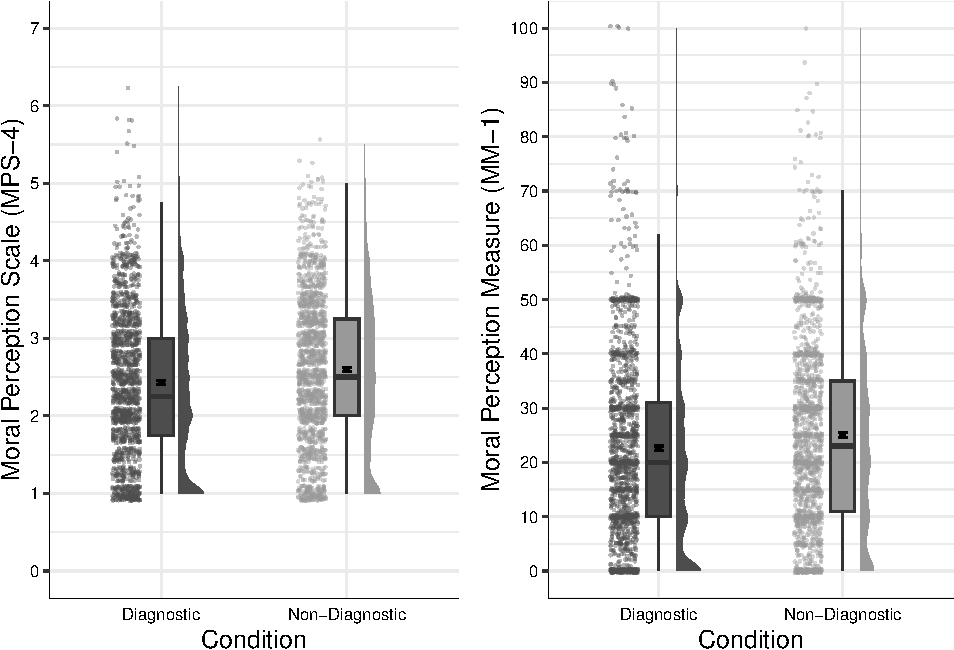
\includegraphics{moral_dilution_in_chunks_files/figure-latex/S1bothconditionplot-1.pdf}
\caption{\label{fig:S1bothconditionplot}Study 1: Differences in moral perception depending on condition}
\end{figure}

We conducted a linear-mixed-effects model to test if condition influenced MM-1 responses. Our outcome measure was MM-1, our predictor variable was condition; we allowed intercepts and the effect of condition to vary across participants. Overall, the model significantly predicted participants responses, and provided a better fit for the data than the baseline model, \(\chi\)\textsuperscript{2}(8) = 475.52, \emph{p} \textless{} .001. Condition significantly predicted MM-1 responses \emph{F}(1, 799.71) = 44.39, \emph{p} \textless{} .001, and when controlling for scenario was a significant predictor in the model \(b\) = -1.22, \emph{t}(799.71) = -6.66, \emph{p} \textless{} .001, with the diagnostic descriptions being rated as more immoral than the non-diagnostic descriptions Figure~\ref{fig:S1bothconditionplot}.

In the supplementary analyses we report the effect of condition on moral perception for each description individually.

\section{Study 2 - Good Characters}\label{study-2---good-characters}

The aim of Study 2 is to test if the dilution effect exists in the moral domain for judgments of morally \emph{good} characters. Participants were presented with descriptions of four characters, two descriptions contain diagnostic information only (morally relevant information) and two will additionally contain non-diagnostic information (non morally relevant information) along with the diagnostic information. We hypothesize that moral perceptions of the diagnostic only descriptions will be more extreme (more moral) than for the descriptions that also contain non-diagnostic information.

\subsection{Study 2: Method}\label{study-2-method}

\subsubsection{Study 2: Participants and design}\label{study-2-participants-and-design}

Study 2 was a within-subjects design. The independent variable was condition with two levels, diagnostic and non-diagnostic. We used the same two dependent variables as in previous studies, the four item moral perception scale (MPS-4, \(\alpha\) = 0.85), and the single item moral perception measure MM-1.

A total sample of 1068 (557 female, 418 male, 13 non-binary, 2 other; 4 prefer not to say, \emph{M}\textsubscript{age} = 29.04, min = 18, max = 74, \emph{SD} = 10.66) started the survey. Participants were recruited from the student population at University of {[}BLINDED{]}.

The majority of participants were from the student body: \emph{n} = 533, (female = 370, male = 147, non-binary/other = 14, prefer not to say 3, \emph{M\textsubscript{age}} = 25.50, \emph{SD} = 9.60).

In order to reach our pre-registered target sample size we recruited additional participants from MTurk: \emph{n} = 287, (female = 96, male = 190, non-binary/other = 1, prefer not to say 1, \emph{M\textsubscript{age}} = 35.70, \emph{SD} = 10.10). Participants from MTurk were paid \$0.40 for their participation.

Participants who failed both manipulation checks were removed (\emph{n} = 248), leaving a total sample of 820 participants (466 female, 337 male, 2 other, 2 prefer not to say; \emph{M}\textsubscript{age} = 29.03, min = 18, max = 74, \emph{SD} = 10.92).

\subsubsection{Study 2: Procedure and materials}\label{study-2-procedure-and-materials}

Again, data were collected using an online questionnaire presented with Qualtrics (www.qualtrics.com). Participants were presented with four descriptions of characters (\emph{Sam}, \emph{Alex}, \emph{Francis}, \emph{Robin} from Pilot Study 2). All descriptions included diagnostic information relating to three moral foundations, e.g., \emph{Imagine a person named Alex. Throughout their life they have been known to protect and provide shelter to the weak and vulnerable, uphold the rights of others, and show respect for authority}. For each participant, two descriptions additionally included non-diagnostic information (this was randomized through blocking, see \color{blue}\url{https://osf.io/mdnpv/?view_only=77883e3fbc3d45f1a35fe92d5318cb67}\color{black}. Study 1 was pre-registered at \color{blue}\url{https://aspredicted.org/NX2_HN6}\color{black}

\subsection{Study 2: Results}\label{study-2-results}

The means and standard deviations for MPS-4 for each scenario are as follows:
\emph{Sam},
\emph{M}\textsubscript{MPS-4} = 6.12, \emph{SD}\textsubscript{MPS-4} = 0.97,
\emph{Francis},
\emph{M}\textsubscript{MPS-4} = 5.86, \emph{SD}\textsubscript{MPS-4} = 1.07,
\emph{Alex},
\emph{M}\textsubscript{MPS-4} = 6.13, \emph{SD}\textsubscript{MPS-4} = 0.99,
\emph{Robin},
\emph{M}\textsubscript{MPS-4} = 6.10, \emph{SD}\textsubscript{MPS-4} = 0.99. There was significant variation depending on the description, \emph{F}(3,2356) = 54.47, \emph{p} \textless{} .001, partial \(\eta\)\textsuperscript{2} = 0.01. \emph{Francis} appeared to be rated as less moral than each of the other characters (all \emph{p}s \textless{} .001).

The means and standard deviations for MM-1 for each scenario are as follows:
\emph{Sam} (diagnostic/moral),
\emph{M}\textsubscript{MM-1} = 84.60, \emph{SD}\textsubscript{MM-1} = 14.47;
\emph{Francis} (diagnostic/moral),
\emph{M}\textsubscript{MM-1} = 82.05, \emph{SD}\textsubscript{MM-1} = 15.24;
\emph{Alex} (diagnostic/moral),
\emph{M}\textsubscript{MM-1} = 85.02, \emph{SD}\textsubscript{MM-1} = 15.01;
\emph{Robin} (diagnostic/moral),
\emph{M}\textsubscript{MM-1} = 84.95, \emph{SD}\textsubscript{MM-1} = 13.94. There was significant variation depending on the description, \emph{F}(3,2387) = 24.20, \emph{p} \textless{} .001, partial \(\eta\)\textsuperscript{2} = 0.007. \emph{Francis} was rated less favorably than all other characters (all \emph{p}s \textless{} .001).

We conducted a linear-mixed-effects model to test if condition influenced MPS-4 responses. Our outcome measure was MPS-4, our predictor variable was condition; we allowed intercepts and the effect of condition to vary across participants, and scenario was also included in the model.
Overall, the model significantly predicted participants responses, and provided a better fit for the data than the baseline model, \(\chi\)\textsuperscript{2}(8) = 160.00, \emph{p} \textless{} .001. Condition did not influence responses to the MPS-4, \emph{F}(1, 838.12) = 0.24, \emph{p} = .624; and was not a significant predictor in the model when controlling for scenario, \(b\) = 0.00, \emph{t}(838) = 0.49, \emph{p} = .624, see Figure~\ref{fig:S2bothconditionplot}.

\begin{figure}
\centering
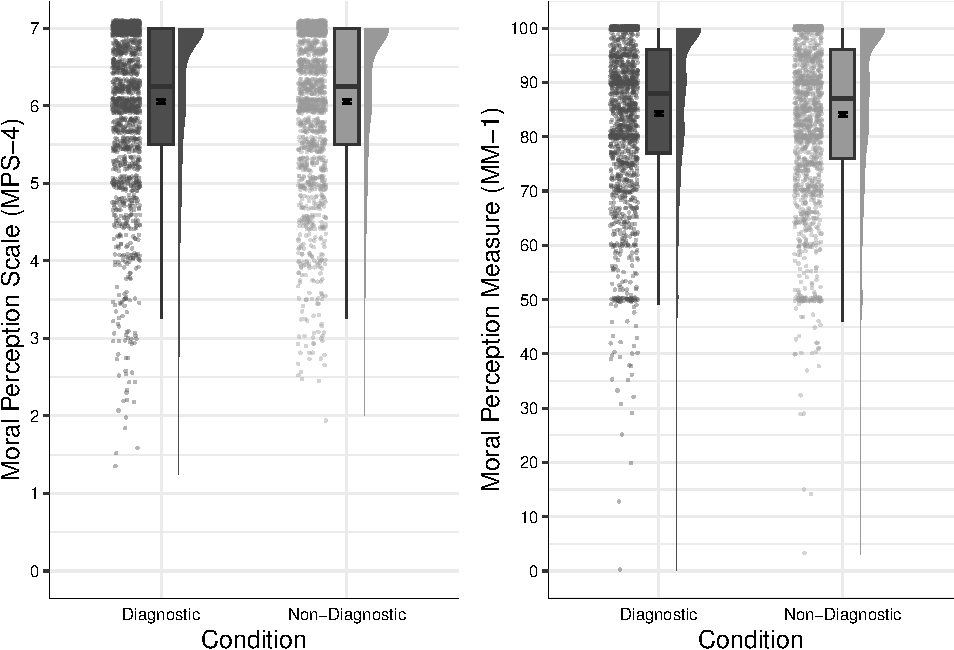
\includegraphics{moral_dilution_in_chunks_files/figure-latex/S2bothconditionplot-1.pdf}
\caption{\label{fig:S2bothconditionplot}Study 2: Differences in moral perception depending on condition}
\end{figure}

We conducted a linear-mixed-effects model to test if condition influenced MM-1 responses. Our outcome measure was MM-1, our predictor variable was condition; we allowed intercepts and the effect of condition to vary across participants. Overall, the model significantly predicted participants responses, and provided a better fit for the data than the baseline model, \(\chi\)\textsuperscript{2}(8) = 75.69, \emph{p} \textless{} .001. Condition did not influence MM-1 responses \emph{F}(1, 2453) = 1.23, \emph{p} = .267, and was not a significant predictor in the model \(b\) = 0.16, \emph{t}(2453) = 1.11, \emph{p} = .267, see Figure~\ref{fig:S2bothconditionplot}.

In the supplementary analyses we report the effect of condition on moral perception for each description individually.

\section{Study 3 - Good and Bad Characters}\label{study-3---good-and-bad-characters}

In Study 1 we found evidence for the moral dilution effect for judgments of \emph{bad} moral characters. In Study 2 we failed replicate this effect for judgments of \emph{good} moral characters. The aim of Study 3 was to test if valence (good vs.~bad) moderates the moral dilution effect. We hypothesized that valence (good vs bad) would interact with condition in producing a dilution effect, such that the dilution effect would be observed for bad characters but not for good characters. Study 3 was pre-registered at \color{blue}\url{https://aspredicted.org/QDF_XT1}\color{black}.

\subsection{Study 3: Method}\label{study-3-method}

\subsubsection{Study 3: Participants and design}\label{study-3-participants-and-design}

Study 3 was a 2 \(\times\) 2 within-subjects factorial design. The first independent variable was condition with two levels, diagnostic and non-diagnostic. The second independent variable was valence of character description, with two levels morally good and morally bad. We used the same two dependent variables as in previous studies, the four item moral perception scale (MPS-4, \(\alpha\) = 0.97), and the single item moral perception measure MM-1.

A total sample of 1386 (535 female, 758 male, 10 non-binary, 2 other; 11 prefer not to say, \emph{M}\textsubscript{age} = 29.67, min = 0.36, max = 70, \emph{SD} = 8.97) started the survey. Participants were recruited from Prolific Academic and paid \$0.40 for their participation.

Participants who failed both manipulation checks (\emph{n} = 541), or did not complete all measures were removed , leaving a total sample of 814 participants (462 female, 327 male, 2 other, 2 prefer not to say; \emph{M}\textsubscript{age} = 26.03, min = 11, max = 70, \emph{SD} = 9.53).

\subsubsection{Study 3: Procedure and materials}\label{study-3-procedure-and-materials}

Again, data were collected using an online questionnaire presented with Qualtrics (www.qualtrics.com). Participants were presented with four descriptions of characters taken from Studies 1 and 2. To ensure consistency across character judgments, we selected descriptions that related to the same moral foundations (care, fairness, and loyalty). We used the same four character names as in previous studies. The \emph{good} characters were \emph{Sam} and \emph{Robin}, and the \emph{bad} characters were \emph{Francis} and \emph{Alex}, e.g., \emph{Imagine a person named Robin. Throughout their life they have been known to show compassion and empathy for others, act with a sense of fairness and justice, and, never to break their word.} or, \emph{Imagine a person named Alex. Throughout their life they have been known to be cruel, act unfairly, and to betray their own group.} Full descriptions for each character are in the supplementary materials. One description for each the \emph{good} and \emph{bad} characters was randomly assigned to include non-diagnostic information for each participant thus all participants were exposed to all conditions (see \color{blue}\url{https://osf.io/mdnpv/?view_only=77883e3fbc3d45f1a35fe92d5318cb67}\color{black} for details of the randomization blocks). Study 3 was pre-registered at \color{blue}\url{https://aspredicted.org/QDF_XT1}\color{black}

\subsection{Study 3: Results}\label{study-3-results}

The means and standard deviations for MPS-4 for each scenario are as follows:
\emph{Sam} (good),
\emph{M}\textsubscript{MPS-4} = 6.20, \emph{SD}\textsubscript{MPS-4} = 0.82,
\emph{Francis} (bad),
\emph{M}\textsubscript{MPS-4} = 2.15, \emph{SD}\textsubscript{MPS-4} = 0.79,
\emph{Alex} (bad),
\emph{M}\textsubscript{MPS-4} = 2.32, \emph{SD}\textsubscript{MPS-4} = 0.88,
\emph{Robin} (good),
\emph{M}\textsubscript{MPS-4} = 6.32, \emph{SD}\textsubscript{MPS-4} = 0.76. There was significant variation depending on the description, \emph{F}(2,1515) = 6,251.52, \emph{p} \textless{} .001, partial \(\eta\)\textsuperscript{2} = 0.86. Both the \emph{good} characters (\emph{Robin} and \emph{Sam}) were rated significantly more favorably than both the \emph{bad} characters (\emph{Alex} and \emph{Francis}; all \emph{p}s \textless{} .001). There were no differences between \emph{Robin} and \emph{Sam} (\emph{good}: \emph{p} = .003) or between \emph{Alex} and \emph{Francis} (\emph{bad}; \emph{p} \textless{} .001).

The means and standard deviations for MM-1 for each scenario are as follows:
\emph{Sam} (good),
\emph{M}\textsubscript{MM-1} = 86.36, \emph{SD}\textsubscript{MM-1} = 13.71;
\emph{Francis} (bad),
\emph{M}\textsubscript{MM-1} = 20.13, \emph{SD}\textsubscript{MM-1} = 16.87;
\emph{Alex} (bad),
\emph{M}\textsubscript{MM-1} = 22.83, \emph{SD}\textsubscript{MM-1} = 17.29;
\emph{Robin} (good),
\emph{M}\textsubscript{MM-1} = 88.41, \emph{SD}\textsubscript{MM-1} = 12.07. There was significant variation depending on the description, \emph{F}(2,1380) = 5,282.47, \emph{p} \textless{} .001, partial \(\eta\)\textsuperscript{2} = 0.826. Again, the \emph{good} characters (\emph{Robin} and \emph{Sam}) were rated significantly more favorably than the \emph{bad} characters (\emph{Alex} and \emph{Francis}; all \emph{p}s \textless{} .001). There were no differences between \emph{Robin} and \emph{Sam} (\emph{good}: \emph{p} = .001) or between \emph{Alex} and \emph{Francis} (\emph{bad}; \emph{p} \textless{} .001).

We conducted a linear-mixed-effects model to test if our predictors influenced MPS-4 responses. Our outcome measure was MPS-4, our predictor variables were condition and valence; we allowed intercepts and the effects of condition and valence to vary across participants.
Overall, the model significantly predicted participants responses, and provided a better fit for the data than the baseline model,
\(\chi\)\textsuperscript{2}(5) = 2,733.13, \emph{p} \textless{} .001.
Overall, there was a significant main effect for condition,
\emph{F}(1, 825) = 47.54, \emph{p} \textless{} .001;
valence significantly predicted responses,
\emph{F}(1, 823) = 3,423.33, \emph{p} \textless{} .001;
and there was a significant condition \(\times\) valence interaction,
\emph{F}(1, 819) = 6.56, \emph{p} = .011.

We conducted a linear-mixed-effects model to test if our predictors influenced MM-1 responses. The model was the same as the previous model, with a change to the outcome measure, our outcome measure for this model was MM-1. As above, our predictor variables were condition and valence; we allowed intercepts and the effects of condition and valence to vary across participants.
Overall, the model significantly predicted participants responses, and provided a better fit for the data than the baseline model,
\(\chi\)\textsuperscript{2}(5) = 6,652.62, \emph{p} \textless{} .001.
Overall there was a main effect for condition,
\emph{F}(1, 829) = 30.29, \emph{p} \textless{} .001;
valence significantly predicted responses,
\emph{F}(1, 824) = 273.59, \emph{p} \textless{} .001;
and there was no significant condition \(\times\) valence interaction,
\emph{F}(1, 825) = 1.57, \emph{p} = .211.

For both MP-4 and MM-1 we found a main effect for condition and valence, and there was a condition \(\times\) valence interaction for MP-4 but not for MM-1. We conducted follow-up analyses to test the if the main effect for condition holds for both good and bad descriptions separately.

\subsection{\texorpdfstring{Differences in the \emph{Bad} Descriptions}{Differences in the Bad Descriptions}}\label{differences-in-the-bad-descriptions}

We conducted a linear-mixed-effects model to test if condition influenced MPS-4 responses. Our outcome measure was MPS-4, our predictor variable was condition; we allowed intercepts and the effect of condition to vary across participants. Overall, the model significantly predicted participants responses, and provided a better fit for the data than the baseline model, \(\chi\)\textsuperscript{2}(3) = 76.88, \emph{p} \textless{} .001. Condition significantly influenced MPS-4 responses \emph{F}(1, 812.00) = 46.02, \emph{p} \textless{} .001, and was a significant predictor in the model \(b\) = -0.10, \emph{t}(812.00) = -6.78, \emph{p} \textless{} .001, see Figure~\ref{fig:S3bothconditionplot}.

We conducted a linear-mixed-effects model to test if condition influenced MM-1 responses. Our outcome measure was MM-1, our predictor variable was condition; we allowed intercepts and the effect of condition to vary across participants. Overall, the model significantly predicted participants responses, and provided a better fit for the data than the baseline model, \(\chi\)\textsuperscript{2}(3) = 46.32, \emph{p} \textless{} .001. Condition significantly influenced MM-1 responses \emph{F}(1, 812.00) = 19.25, \emph{p} \textless{} .001, and was a significant predictor in the model \(b\) = -1.14, \emph{t}(812.00) = -4.39, \emph{p} \textless{} .001, see Figure~\ref{fig:S3bothconditionplot}.

\subsection{\texorpdfstring{Differences in the \emph{Good} Descriptions}{Differences in the Good Descriptions}}\label{differences-in-the-good-descriptions}

We conducted a linear-mixed-effects model to test if condition influenced MPS-4 responses. Our outcome measure was MPS-4, our predictor variable was condition; we allowed intercepts and the effect of condition to vary across participants. Overall, the model significantly predicted participants responses, and provided a better fit for the data than the baseline model, \(\chi\)\textsuperscript{2}(3) = 30.01, \emph{p} \textless{} .001. Condition significantly influenced MPS-4 responses \emph{F}(1, 812.00) = 11.87, \emph{p} \textless{} .001, and was a significant predictor in the model \(b\) = 0.05, \emph{t}(812.00) = 3.45, \emph{p} \textless{} .001, see Figure~\ref{fig:S3bothconditionplot}.

\begin{figure}
\centering
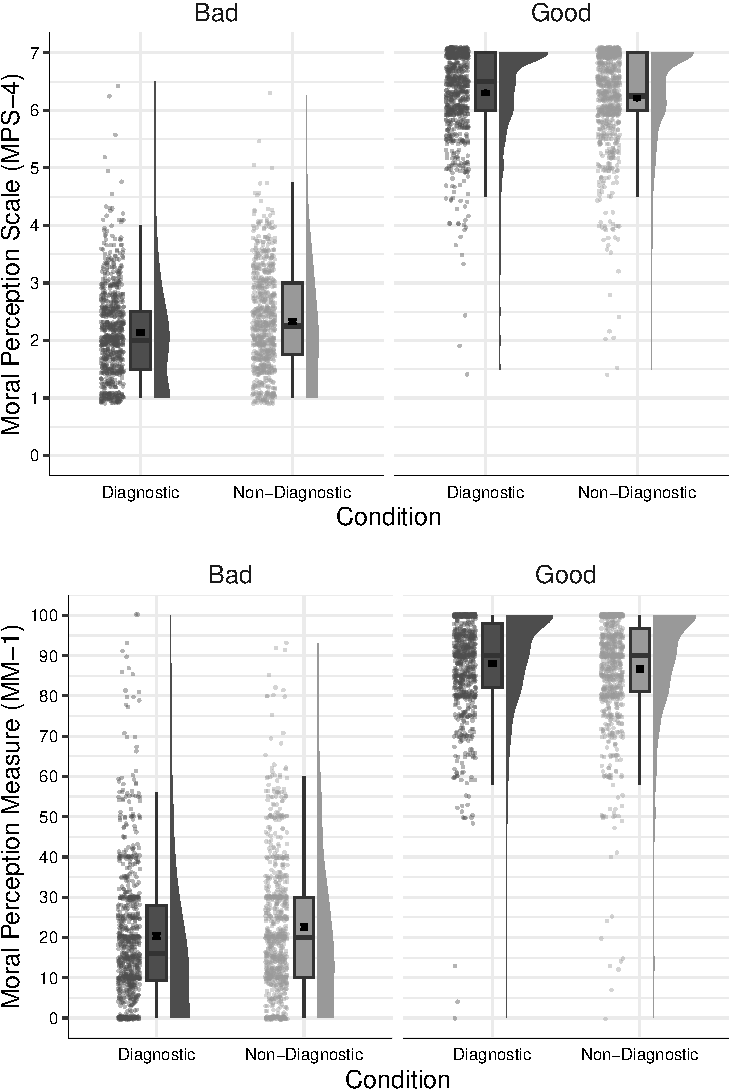
\includegraphics{moral_dilution_in_chunks_files/figure-latex/S3bothconditionplot-1.pdf}
\caption{\label{fig:S3bothconditionplot}Study 3: Differences in moral perception depending on condition}
\end{figure}

We conducted a linear-mixed-effects model to test if condition influenced MM-1 responses. Our outcome measure was MM-1, our predictor variable was condition; we allowed intercepts and the effect of condition to vary across participants. Overall, the model significantly predicted participants responses, and provided a better fit for the data than the baseline model, \(\chi\)\textsuperscript{2}(3) = 41.07, \emph{p} \textless{} .001. Condition significantly influenced MM-1 responses \emph{F}(1, 812) = 13.21, \emph{p} \textless{} .001, and was a significant predictor in the model \(b\) = 0.69, \emph{t}(812) = 3.63, \emph{p} \textless{} .001, see Figure~\ref{fig:S3bothconditionplot}.

\newpage

\section{Aggregate Results}\label{aggregate-results}

A mini meta-analysis and found a significant dilution effect across both good and bad character descriptions across all studies \(\chi\)\textsuperscript{2}(16) = 114.11, \emph{p} \textless{} .001 (Fisher's method); or when weighting for sample size, \emph{z} = 7.995, \emph{p} \textless{} .001 (Stouffer's Z-score method).

A mini meta-analysis and found a significant dilution effect for bad character descriptions across all studies \(\chi\)\textsuperscript{2}(8) = 73.68, \emph{p} \textless{} .001 (Fisher's method); or when weighting for sample size, \emph{z} = 7.438, \emph{p} \textless{} .001 (Stouffer's Z-score method).

A mini meta-analysis and found a significant dilution effect for good character descriptions across all studies \(\chi\)\textsuperscript{2}(8) = 40.43, \emph{p} \textless{} .001 (Fisher's method); or when weighting for sample size, \emph{z} = 3.871, \emph{p} \textless{} .001 (Stouffer's Z-score method).

\section{Discussion}\label{discussion}

\section{Accessibility Statement}\label{accessibility-statement}

All data and analysis code are publicly available on this project's OSF page at \color{blue}\url{https://osf.io/mdnpv/?view_only=77883e3fbc3d45f1a35fe92d5318cb67}\color{black}.

\newpage

\section{References}\label{references}


\phantomsection\label{refs}
\begin{CSLReferences}{1}{0}
\bibitem[\citeproctext]{ref-cameron_morality_2013}
Cameron, C. D., Payne, B. K., \& Doris, J. M. (2013). Morality in high definition: {Emotion} differentiation calibrates the influence of incidental disgust on moral judgments. \emph{Journal of Experimental Social Psychology}, \emph{49}(4), 719--725. \url{https://doi.org/10.1016/j.jesp.2013.02.014}

\bibitem[\citeproctext]{ref-christensen_moral_2014}
Christensen, J. F., Flexas, A., Calabrese, M., Gut, N. K., \& Gomila, A. (2014). Moral judgment reloaded: A moral dilemma validation study. \emph{Frontiers in Psychology}, \emph{5}, 1--18. \url{https://doi.org/10.3389/fpsyg.2014.00607}

\bibitem[\citeproctext]{ref-christensen_moral_2012}
Christensen, J. F., \& Gomila, A. (2012). Moral dilemmas in cognitive neuroscience of moral decision-making: {A} principled review. \emph{Neuroscience \& Biobehavioral Reviews}, \emph{36}(4), 1249--1264. \url{https://doi.org/10.1016/j.neubiorev.2012.02.008}

\bibitem[\citeproctext]{ref-giner-sorolla_functional_2018}
Giner-Sorolla, R. (2018). A {Functional Conflict Theory} of {Moral Emotions}. In K. J. Gray \& J. Graham (Eds.), \emph{Atlas of {Moral Psychology}} (pp. 81--87). {New York, NY}: {The Guilford Press}.

\bibitem[\citeproctext]{ref-gray_impure_2015}
Gray, K. J., \& Keeney, J. E. (2015). Impure or {Just Weird}? {Scenario Sampling Bias Raises Questions About} the {Foundation} of {Morality}. \emph{Social Psychological and Personality Science}, \emph{6}(8), 859--868. \url{https://doi.org/10.1177/1948550615592241}

\bibitem[\citeproctext]{ref-gray_moral_2012}
Gray, K. J., Waytz, A., \& Young, L. (2012). The {Moral Dyad}: {A Fundamental Template Unifying Moral Judgment}. \emph{Psychological Inquiry}, \emph{23}(2), 206--215. \url{https://doi.org/10.1080/1047840X.2012.686247}

\bibitem[\citeproctext]{ref-greene_fmri_2001}
Greene, J. D., Sommerville, R. B., Nystrom, L. E., Darley, J. M., \& Cohen, J. D. (2001). An {fMRI} investigation of emotional engagement in moral judgment. \emph{Science (New York, N.Y.)}, \emph{293}(5537), 2105--2108. \url{https://doi.org/10.1126/science.1062872}

\bibitem[\citeproctext]{ref-igou_conversational_2005}
Igou, E. R., \& Bless, H. (2005). The {Conversational Basis} for the {Dilution Effect}. \emph{Journal of Language and Social Psychology}, \emph{24}(1), 25--35. \url{https://doi.org/10.1177/0261927X04273035}

\bibitem[\citeproctext]{ref-kahneman_subjective_1972}
Kahneman, D., \& Tversky, A. (1972). Subjective probability: {A} judgment of representativeness. \emph{Cognitive Psychology}, \emph{3}(3), 430--454. \url{https://doi.org/10.1016/0010-0285(72)90016-3}

\bibitem[\citeproctext]{ref-labella_dilution_2004}
LaBella, C., \& Koehler, D. J. (2004). Dilution and confirmation of probability judgments based on nondiagnostic evidence. \emph{Memory and Cognition}, \emph{32}(7), 1076--1089. \url{https://doi.org/10.3758/BF03196883}

\bibitem[\citeproctext]{ref-mchugh_moral_2022}
McHugh, C., McGann, M., Igou, E. R., \& Kinsella, E. L. (2022). Moral {Judgment} as {Categorization} ({MJAC}). \emph{Perspectives on Psychological Science}, \emph{17}(1), 131--152. \url{https://doi.org/10.1177/1745691621990636}

\bibitem[\citeproctext]{ref-meyvis_consumers_2002}
Meyvis, T., \& Janiszewski, C. (2002). Consumers' {Beliefs} about {Product Benefits}: {The Effect} of {Obviously Irrelevant Product Information}. \emph{Journal of Consumer Research}, \emph{28}(4), 618--635. \url{https://doi.org/10.1086/338205}

\bibitem[\citeproctext]{ref-nisbett_dilution_1981}
Nisbett, R. E., Zukier, H., \& Lemley, R. E. (1981). The dilution effect: {Nondiagnostic} information weakens the implications of diagnostic information. \emph{Cognitive Psychology}, \emph{13}(2), 248--277. \url{https://doi.org/10.1016/0010-0285(81)90010-4}

\bibitem[\citeproctext]{ref-schein_theory_2018}
Schein, C., \& Gray, K. J. (2018). The {Theory} of {Dyadic Morality}: {Reinventing Moral Judgment} by {Redefining Harm}. \emph{Personality and Social Psychology Review}, \emph{22}(1), 32--70. \url{https://doi.org/10.1177/1088868317698288}

\bibitem[\citeproctext]{ref-zukier_dilution_1982}
Zukier, H. (1982). The dilution effect: {The} role of the correlation and the dispersion of predictor variables in the use of nondiagnostic information. \emph{Journal of Personality and Social Psychology}, \emph{43}(6), 1163--1174. \url{https://doi.org/10.1037/0022-3514.43.6.1163}

\end{CSLReferences}

\end{document}
